%\immediate\write18{tex penrose_code.dtx}
%\immediate\write18{cd ../spath3; tex spath3_code.dtx}
\documentclass{article}
\RequirePackage[enable-debug]{expl3}
\ExplSyntaxOn
\debug_on:n {check-declarations, deprecation}
\ExplSyntaxOff

\usepackage[svgnames]{xcolor}
\usepackage{tikz}
\usetikzlibrary{
  tilings.penrose,
  tilings.polykite,
  calc
}

\tikzset{
  every tile pic/.style={draw,ultra thick},
  every circle arc/.style={draw,thin},
  every long arc/.style={draw,thin},
}

\makeatletter
\tikzset{
  tint fill colour/.code={%
    \edef\@temp{%
      \def\noexpand\tikz@fillcolor{\tikz@fillcolor!#1}%
      \noexpand\tikz@addoption{\noexpand\pgfsetfillcolor{\tikz@fillcolor!#1}}%
    }%
    \@temp
  }
}
\makeatother

\colorlet{thinRhombus}{DarkOrchid}
\colorlet{thickRhombus}{DarkSlateGray}
\colorlet{circleArc}{RosyBrown}
\colorlet{longArc}{LawnGreen}

\colorlet{kite}{HotPink}
\colorlet{dart}{Fuchsia}

\colorlet{goldenTriangle}{Gold}
\colorlet{reverseGoldenTriangle}{Magenta}
\colorlet{goldenGnomon}{Cyan}
\colorlet{reverseGoldenGnomon}{LimeGreen}


\begin{document}

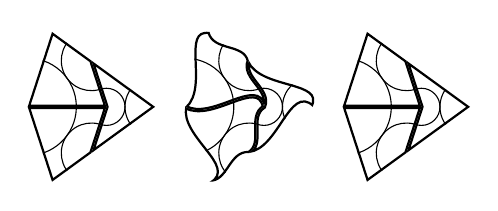
\begin{tikzpicture}
\pic[draw,dart,name=dart];
\pic[draw,kite,align with=dart along c];
\pic[draw,kite,align with=dart along C];
\tikzset{clone tile path={original kite}{kite}}
\tikzset{clone tile path={original dart}{dart}}
\path[save tiling path=a] (0,0) to[out=-30,in=100] (1,0);
\path[save tiling path=c] (0,0) to[out=-40,in=140] (1,0);
\BakeTile{kite}
\BakeTile{dart}
\pic[xshift=2cm,draw,dart,name=dart];
\pic[draw,kite,align with=dart along c];
\pic[draw,kite,align with=dart along C];
\tikzset{clone tile path={kite}{original kite}}
\tikzset{clone tile path={dart}{original dart}}
\pic[xshift=4cm,draw,dart,name=dart];
\pic[draw,kite,align with=dart along c];
\pic[draw,kite,align with=dart along C];
\end{tikzpicture}


\DefineTile {square}{a A a A}
{
  {0,0}
  {1,0}
  {1,1}
  {0,1}
}

\begin{tikzpicture}
\path[save tiling path=a] (0,0) to[out=45,in=135] (1,0);
\BakeTile{square}
\pic[square,name=A,fill=green];
\foreach \edg/\col in {a1/cyan, A1/magenta, a2/orange, A2/pink}
{
  \fill[\col] (0,0) (A-edge \edg\space start) circle[radius=3pt];
}
\pic[square,align with=A along a1 using 1,name=B,fill=red];
\pic[square,align with=A along A1 using 2,fill=red];
\pic[square,align with=A along A2 using 1,fill=red];
\pic[square,align with=B along a1 using 2,fill=green];
\pic[square,align with=B along a2 using 1,fill=green];
\end{tikzpicture}


\begin{tikzpicture}
\path[save tiling path=a] (0,0) -- (.3,-.1) to[out=30,in=200] (1,0);
\path[save tiling path=b] (0,0) -- (.3,-.1) to[out=30,in=180] (1,0);
\path[save tiling path=c] (0,0) -- (.3,-.1) to[out=30,in=160] (1,0);
\path[save tiling path=d] (0,0) -- (.3,-.1) to[out=30,in=140] (1,0);
\path[save tiling path=e] (0,0) -- (.3,-.1) to[out=30,in=120] (1,0);
\BakeTile{kite}
\BakeTile{dart}
\BakeTile{thin rhombus}
\BakeTile{thick rhombus}
\BakeTile{pentagon 5}
\BakeTile{pentagon 3}
\BakeTile{pentagon 2}
\BakeTile{pentagram}
\BakeTile{boat}
\BakeTile{diamond}
\BakeTile{golden triangle}
\BakeTile{reverse golden triangle}
\BakeTile{golden gnomon}
\BakeTile{reverse golden gnomon}
\end{tikzpicture}

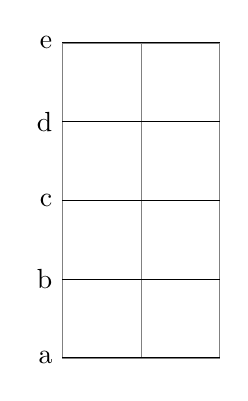
\begin{tikzpicture}
\draw[help lines] (0,1) grid (2,5);
\foreach[count=\k] \pth in {a,b,c,d,e}
{
  \node[left] at (0, \k) {\pth};
  \draw[spath/set name=tiling side, spath/transform globally={\pth}{yshift=\k cm, scale=1cm/1pt}, spath/restore=\pth];
}
\foreach[count=\k] \pth in {A,B,C,D,E}
{
  \draw[
    spath/set name=tiling side,
    spath/transform globally={\pth}{yshift=\k cm, xshift= 1cm, scale=1cm/1pt},
    spath/restore=\pth
  ];
}
\end{tikzpicture}

\section{Kites and Darts}

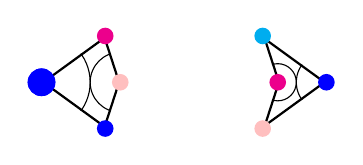
\begin{tikzpicture}
\pic[kite,name=tile];
\fill[blue] (0,0) circle[radius=5pt];
\foreach \edg/\col/\opp in {a/cyan/A, c/magenta/C, A/blue/a, C/pink/c}
{
  \fill[\col] (0,0) (tile-edge \edg\space start) circle[radius=3pt];
}
\pic[every tile pic, name=tile] at (3,0) {dart};
\fill[blue] (0,0) circle[radius=5pt];
\foreach \edg/\col/\opp in {a/cyan/A, c/magenta/C, A/blue/a, C/pink/c}
{
  \fill[\col] (0,0) (tile-edge \edg\space start) circle[radius=3pt];
}
\end{tikzpicture}

\subsection{Alignments}

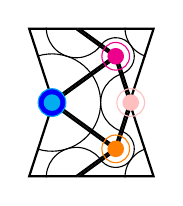
\begin{tikzpicture}
\pic[kite,name=tile];
\pic[dart,align with=tile along c, name=ctile];
\pic[kite,align with=tile along a, name=atile];
\pic[kite,align with=tile along A, name=Atile];
\pic[dart,align with=tile along C, name=Ctile];
\fill[blue] (0,0) circle[radius=5pt];
\foreach \edg/\col/\opp in {a/cyan/A, c/magenta/C, A/orange/a, C/pink/c}
{
  \fill[\col] (0,0) (tile-edge \edg\space start) circle[radius=3pt];
  \draw[\col] (0,0) (\edg tile-edge \opp\space end) circle[radius=5pt];
}
\end{tikzpicture}

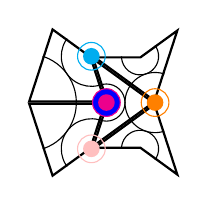
\begin{tikzpicture}
\pic[dart,name=tile];
\pic[kite,align with=tile along c, name=ctile];
\pic[dart,align with=tile along a, name=atile];
\pic[dart,align with=tile along A, name=Atile];
\pic[kite,align with=tile along C, name=Ctile];
\fill[blue] (0,0) circle[radius=5pt];
\foreach \edg/\col/\opp in {a/cyan/A, c/magenta/C, A/orange/a, C/pink/c}
{
  \fill[\col] (0,0) (tile-edge \edg\space start) circle[radius=3pt];
  \draw[\col] (0,0) (\edg tile-edge \opp\space end) circle[radius=5pt];
}
\end{tikzpicture}

\subsection{Decomposition}

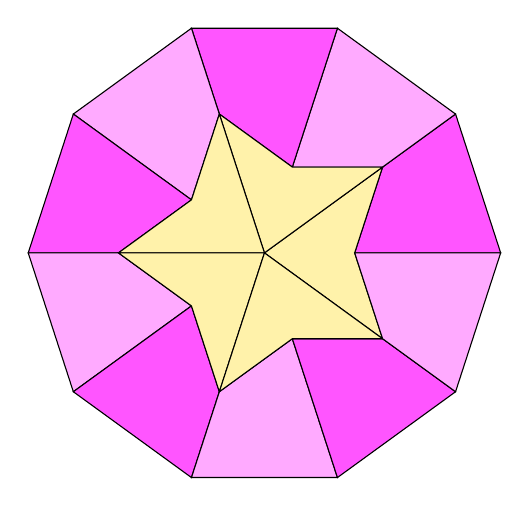
\begin{tikzpicture}[
  every tile/.style={draw},
  every golden triangle/.style={fill=goldenTriangle},
  every reverse golden triangle/.style={fill=reverseGoldenTriangle},
  every golden gnomon/.style={fill=goldenGnomon},
  every reverse golden gnomon/.style={fill=reverseGoldenGnomon},
  every kite/.style={fill=reverseGoldenTriangle},
  every dart/.style={fill=goldenTriangle},
  tile/.code 2 args={
    \pgfmathsetmacro\tint{100*(1 - #1/(1.5*#2))}
    \pgfkeysalso{tint fill colour=\tint}
%    \message{#1 and #2,}
  }
]
\foreach[evaluate=\k as \mk using {\k+Mod(\k,2)},evaluate=\k as \ax using {Mod(\k,2) == 0 ? "T" : "t"}] \k in {0,...,9} {
  \begin{scope}[rotate=\mk*36]
  \TilingDecomposition[tiling step=3cm]{kite}{1}{\ax}
  \end{scope}
}
\end{tikzpicture}


\section{Rhombii}

\subsection{Alignments}

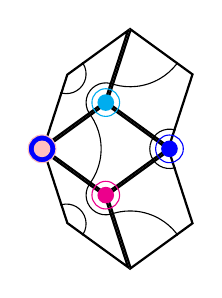
\begin{tikzpicture}
\pic[thick rhombus,name=tile];
\pic[thin rhombus,align with=tile along b, name=btile];
\pic[thick rhombus,align with=tile along a, name=atile];
\pic[thick rhombus,align with=tile along A, name=Atile];
\pic[thin rhombus,align with=tile along B, name=Btile];
\fill[blue] (0,0) circle[radius=5pt];
\foreach \edg/\col/\opp in {a/cyan/A, b/magenta/B, A/blue/a, B/pink/b}
{
  \fill[\col] (0,0) (tile-edge \edg\space start) circle[radius=3pt];
  \draw[\col] (0,0) (\edg tile-edge \opp\space end) circle[radius=5pt];
}
\end{tikzpicture}

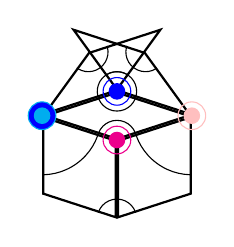
\begin{tikzpicture}
\pic[thin rhombus,name=tile];
\pic[thick rhombus,align with=tile along b, name=btile];
\pic[thin rhombus,align with=tile along a, name=atile];
\pic[thin rhombus,align with=tile along A, name=Atile];
\pic[thick rhombus,align with=tile along B, name=Btile];
\fill[blue] (0,0) circle[radius=5pt];
\foreach \edg/\col/\opp in {a/cyan/A, b/magenta/B, A/blue/a, B/pink/b}
{
  \fill[\col] (0,0) (tile-edge \edg\space start) circle[radius=3pt];
  \draw[\col] (0,0) (\edg tile-edge \opp\space end) circle[radius=5pt];
}
\end{tikzpicture}

\subsection{Decomposition}

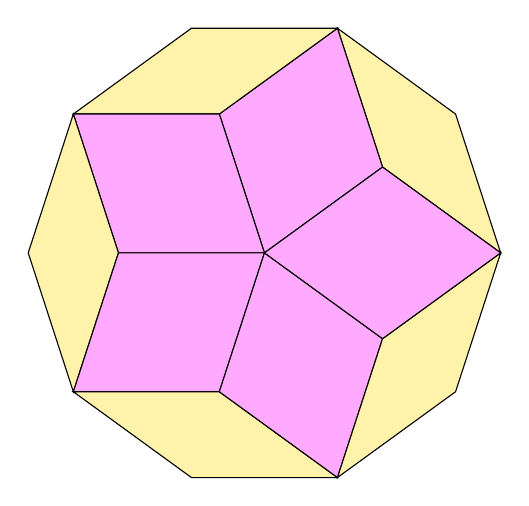
\begin{tikzpicture}[
  every tile/.style={draw},
  every golden triangle/.style={fill=goldenTriangle},
  every reverse golden triangle/.style={fill=reverseGoldenTriangle},
  every golden gnomon/.style={fill=goldenGnomon},
  every reverse golden gnomon/.style={fill=reverseGoldenGnomon},
  every thick rhombus/.style={fill=reverseGoldenTriangle},
  every thin rhombus/.style={fill=goldenTriangle},
  tile/.code 2 args={
    \pgfmathsetmacro\tint{100*(1 - #1/(1.5*#2))}
    \pgfkeysalso{tint fill colour=\tint}
%    \message{#1 and #2,}
  }
]
\foreach[evaluate=\k as \mk using {\k+Mod(\k,2)},evaluate=\k as \ax using {Mod(\k,2) == 0 ? "T" : "t"}] \k in {0,...,9} {
  \begin{scope}[rotate=\mk*36]
  \TilingDecomposition[tiling step=3cm]{rhombus}{1}{\ax}
  \end{scope}
}
\end{tikzpicture}





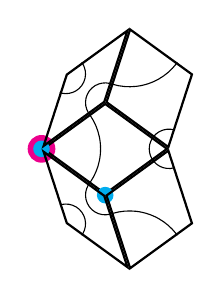
\begin{tikzpicture}
\fill[magenta] (0,0) circle[radius=5pt];
\pic[thick rhombus,name=tile];
\fill[cyan] (0,0) (tile-edge b start) circle[radius=3pt];
\fill[cyan] (0,0) (tile-edge b end) circle[radius=3pt];
\pic[thin rhombus,align with=tile along b];
\pic[thick rhombus,align with=tile along a];
\pic[thick rhombus,align with=tile along A];
\pic[thin rhombus,align with=tile along B];
\end{tikzpicture}

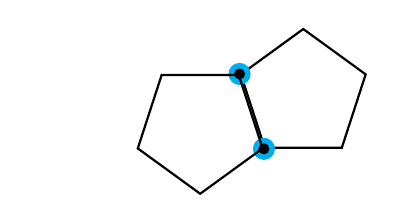
\begin{tikzpicture}
\pic[pentagon 5,name=ptile,at={(3,0)}];
\fill[cyan] (0,0) (ptile-edge a1 start) circle[radius=4pt];
\fill[cyan] (0,0) (ptile-edge a1 end) circle[radius=4pt];
\pic[pentagon 3,align with=ptile along a1,name=qtile];
\fill (0,0) (qtile-edge A start) circle[radius=2pt];
\fill (0,0) (qtile-edge A end) circle[radius=2pt];
\end{tikzpicture}

\section{Polykites}

\tikzset{
  hexagon/.pic={
    \path[pic actions] (1,0)
    foreach \k in {1,...,6} { -- (\k*60:1)}
    foreach \k in {1,...,6} {(0,0) -- (\k*60:1)}
    foreach \k in {1,...,6} {(0,0) -- (\k*60+30:{sqrt(3)/2})}
    ;
  },
  every tile/.style={draw}
}

\pgfmathsetmacro\hatsf{1/sqrt(8)}
\pgfmathsetmacro\grat{(1 + sqrt(5))/2}

\begin{tikzpicture}[
  every aperiodical hat/.style={
    draw,
    ultra thick
  },
]
\pic[draw=none,fill=gray!50] {aperiodical hat};
\pic[draw,gray] at (-1,0) {hexagon};
\pic[draw,gray] at (60:1) {hexagon};
\pic[draw,gray] at (-60:1) {hexagon};
\pic[aperiodical hat,name=hat-a];
\pic[aperiodical hat,name=hat-b,align with=hat-a along 11 using 4];
\pic[aperiodical hat,name=hat-c,align with=hat-a along 26 using 7];
\pic[aperiodical hat,name=hat-d,align with=hat-a along 24 using 5];
\pic[aperiodical hat,name=hat-e,align with=hat-a along 13 using 2];
\pic[aperiodical hat,name=hat-f,align with=hat-a along 16 using 5];
\pic[red,flip tile,aperiodical hat,name=hat-g,align with=hat-a along 21 using 3];
\pic[aperiodical hat,name=hat-h,align with=hat-g back along 14 using 6];
\end{tikzpicture}


\begin{tikzpicture}
\pic[super cluster T,name=super t];
\foreach \side in {A1,A2,b}
{
  \draw[red] (super t-edge \side\space start) circle[radius=3pt];
  \draw[blue] (super t-edge \side\space end) circle[radius=5pt];
  \path  (super t-edge \side\space start) -- node[fill=white] {\(\side\)}  (super t-edge \side\space end);
}
\draw[red,->|] (super t-edge b start) -- +(60:3*\grat);
\end{tikzpicture}

\begin{tikzpicture}
\pic[super cluster H,name=super h];
\foreach \side in {d1,d2,d3,D1,D2,D3,B1,B2,a}
{
  \draw[red] (super h-edge \side\space start) circle[radius=3pt];
  \draw[blue] (super h-edge \side\space end) circle[radius=5pt];
  \path  (super h-edge \side\space start) -- node[fill=white] {\(\side\)}  (super h-edge \side\space end);
}
\draw[red,->|] (super h-edge B1 start) -- +(240:1+3*\grat);
\end{tikzpicture}

\begin{tikzpicture}
\pic[super cluster P,name=super p];
\foreach \side in {A,11,D1,d1,b,12,D2,d2}
{
  \draw[red] (super p-edge \side\space start) circle[radius=3pt];
  \draw[blue] (super p-edge \side\space end) circle[radius=5pt];
  \path  (super p-edge \side\space start) -- node[fill=white] {\(\side\)}  (super p-edge \side\space end);
}
\draw[red,->|] (super p-edge b start) -- +(180:3*\grat);
\end{tikzpicture}

\begin{tikzpicture}
\pic[super cluster F,name=super f];
\foreach \side in {11,12,D1,D2,d1,d2,c,C,b}
{
  \draw[red] (super f-edge \side\space start) circle[radius=3pt];
  \draw[blue] (super f-edge \side\space end) circle[radius=5pt];
  \path  (super f-edge \side\space start) -- node[fill=white] {\(\side\)}  (super f-edge \side\space end);
}
\draw[red,->|] (super f-edge b start) -- +(180:3*\grat);
\draw[blue] (super f-edge D1 end) -- (super f-edge d1 start);
\draw[blue] ($(super f-edge D1 end)!.5!(super f-edge d1 start)$) -- ($($(super f-edge D1 end)!.5!(super f-edge d1 start)$)!{1/sqrt(3)}!90:(super f-edge D1 end)$);
\end{tikzpicture}



\begin{tikzpicture}[every tile/.style={draw}]

\begin{scope}
\fill[blue] (0,0) circle[radius=3pt];
\pic[ultra thick,red,meta cluster T,at={(0,0)},name=a];
\path (a-edge b start) -- node {\(b\)} (a-edge b end);
\pic[scale=\hatsf,meta cluster H,at={(0,0)},name=h-tile];
\pic[meta cluster P, align with=h-tile along B1];
\pic[meta cluster P, align with=h-tile along B2];
\end{scope}

\begin{scope}[yshift=-5cm]
\pic[ultra thick,red,meta cluster H,at={(0,0)},name=h-tile];
\foreach \side in {a,D1,d1,B1,D2,d2,B2,D3,d3}
{
  \draw[red] (h-tile-edge \side\space start) circle[radius=3pt];
  \draw[blue] (h-tile-edge \side\space end) circle[radius=5pt];
}
\begin{scope}
\pic[meta cluster T,at={(0,0)},rotate=180,name=t-tile,scale=\hatsf];
\pic[meta cluster H,align with=t-tile along b using 1,name=h-tile-1];
\pic[meta cluster H,align with=t-tile along A1,name=h-tile-2];
\pic[meta cluster H,align with=t-tile along A2,name=h-tile-3];
\pic[meta cluster P,align with=h-tile-2 along B2];
\pic[meta cluster P,align with=h-tile-3 along B2];
\pic[meta cluster F,align with=h-tile-1 along B2];
\pic[meta cluster F,align with=h-tile-2 along B1];
\pic[meta cluster F,align with=h-tile-3 along B1];
\end{scope}

\end{scope}
\end{tikzpicture}


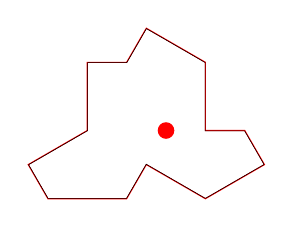
\begin{tikzpicture}
\fill[red] (0,0) circle[radius=3pt];
\draw[red,scale=.5] (1,0)
    ++(90 : {sqrt(3)}) --
    ++(150 : {sqrt(3)}) --
    ++(240 : 1) --
    ++(180 : 1) --
    ++(-90 : {sqrt(3)}) --
    ++(210 : {sqrt(3)}) --
    ++(-60 : 1) --
    ++(0 : 1) --
    ++(0 : 1) --
    ++(60 : 1) --
    ++(-30 : {sqrt(3)}) --
    ++(30 : {sqrt(3)}) --
    ++(120 : 1) --
    ++(180 : 1) -- cycle
;
\pic[draw] {aperiodical hat};
\end{tikzpicture}


\begin{tikzpicture}[overlay]
\path[save tiling path=1] (0,0) to[out=36,in=180+36] (1,0);
\path[save tiling path=2] (0,0) to[out=-18,in=180-18] (1,0);
\end{tikzpicture}

%\BakeTile{aperiodical hat}

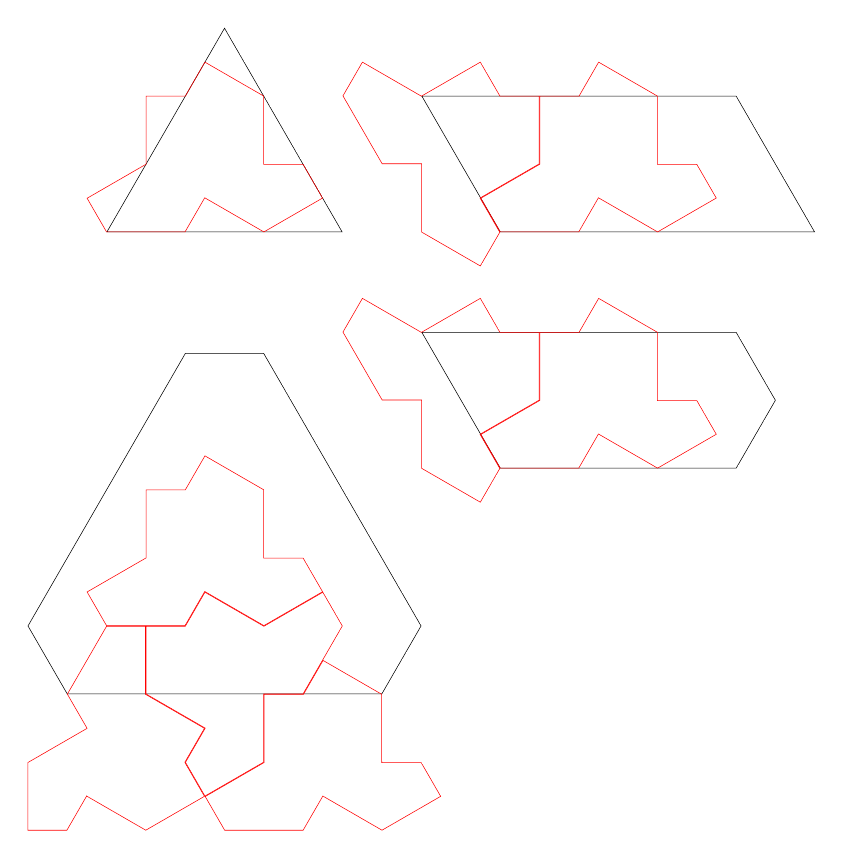
\begin{tikzpicture}[
  every tile/.style={draw},
]
\pic {meta cluster T};
\pic[red] {aperiodical hat};

\pic at (5,0) {meta cluster P};
\pic[red] at (5,0) (p-hat-a) {aperiodical hat};
\pic[red,align with=p-hat-a along 13 using 2] {aperiodical hat};

\begin{scope}[yshift=-3cm]
\pic at (5,0) {meta cluster F};
\pic[red] at (5,0) (f-hat-a) {aperiodical hat};
\pic[red,align with=f-hat-a along 13 using 2] {aperiodical hat};
\end{scope}
\begin{scope}[yshift=-5cm]
\pic {meta cluster H};
\pic[red] (h-hat-a) {aperiodical hat};
\pic[red,name=h-hat-b,align with=h-hat-a along 24 using 3] {aperiodical hat};
\pic[red,flip tile,name=h-hat-c,align with=h-hat-a along 25 using 1] {aperiodical hat};
\pic[red,name=h-hat-d,align with=h-hat-c back along 15 using 3] {aperiodical hat}; 
\end{scope}
\end{tikzpicture}




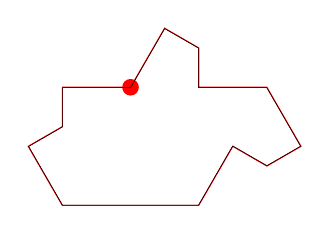
\begin{tikzpicture}
\fill[red] (0,0) circle[radius=3pt];
\draw[red,scale=.5] ({sqrt(3)},0)
    ++(90 : 1) --
    ++(150 : 1) --
    ++(240 : {sqrt(3)}) --
    ++(180 : {sqrt(3)}) --
    ++(-90 : 1) --
    ++(210 : 1) --
    ++(-60 : {sqrt(3)}) --
    ++(0 : {sqrt(3)}) --
    ++(0 : {sqrt(3)}) --
    ++(60 : {sqrt(3)}) --
    ++(-30 : 1) --
    ++(30 : 1) --
    ++(120 : {sqrt(3)}) --
    ++(180 : {sqrt(3)}) -- cycle
;
\pic[draw] {aperiodical turtle};
\end{tikzpicture}


\begin{tikzpicture}[overlay]
\path[save tiling path=1] (0,0) to[out=36,in=180+36] (1,0);
\path[save tiling path=2] (0,0) to[out=-18,in=180-18] (1,0);
\end{tikzpicture}

%\BakeTile{aperiodical turtle}

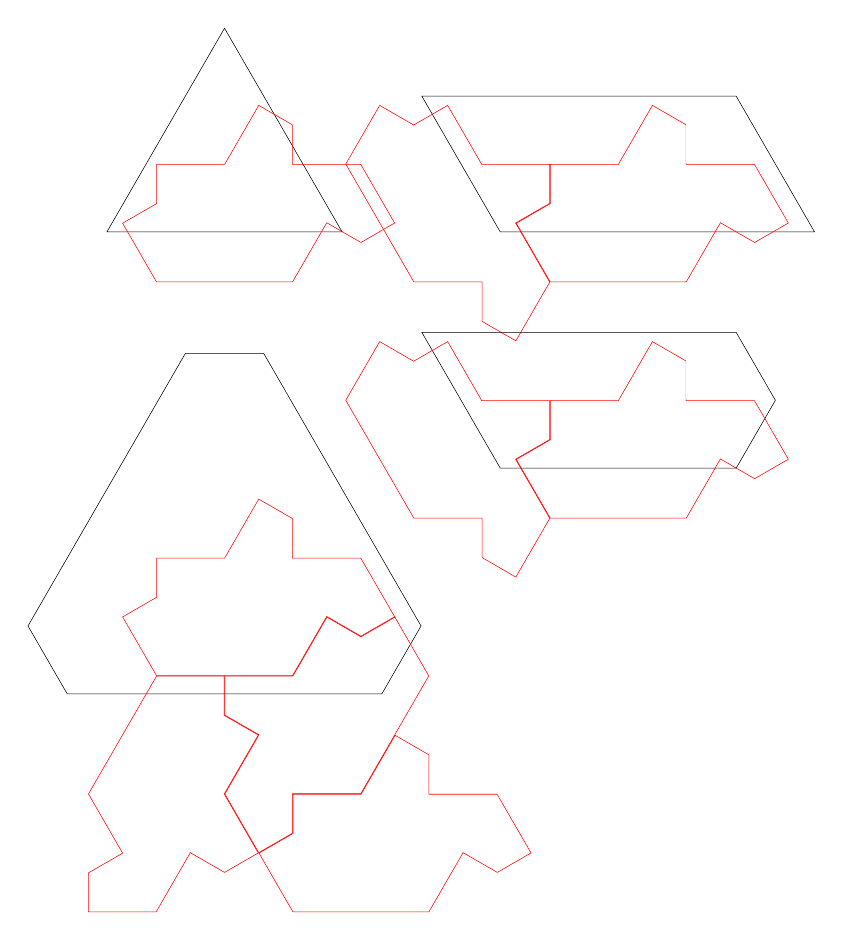
\begin{tikzpicture}[
  every tile/.style={draw},
]
\pic {meta cluster T};
\pic[red] {aperiodical turtle};

\pic at (5,0) {meta cluster P};
\pic[red] at (5,0) (p-turtle-a) {aperiodical turtle};
\pic[red,align with=p-turtle-a along 13 using 2] {aperiodical turtle};

\begin{scope}[yshift=-3cm]
\pic at (5,0) {meta cluster F};
\pic[red] at (5,0) (f-turtle-a) {aperiodical turtle};
\pic[red,align with=f-turtle-a along 13 using 2] {aperiodical turtle};
\end{scope}
\begin{scope}[yshift=-5cm]
\pic {meta cluster H};
\pic[red] (h-turtle-a) {aperiodical turtle};
\pic[red,name=h-turtle-b,align with=h-turtle-a along 24 using 3] {aperiodical turtle};
\pic[red,flip tile,name=h-turtle-c,align with=h-turtle-a along 25 using 1] {aperiodical turtle};
\pic[red,name=h-turtle-d,align with=h-turtle-c back along 15 using 3] {aperiodical turtle}; 
\end{scope}
\end{tikzpicture}

\begin{tikzpicture}[
  every aperiodical turtle/.style={
    draw,
    ultra thick
  },
]
\pic[draw=none,fill=gray!50] {aperiodical turtle};
\pic[draw,gray] at (-1,0) {hexagon};
\pic[draw,gray] at (60:1) {hexagon};
\pic[draw,gray] at (-60:1) {hexagon};
\pic[aperiodical turtle,name=turtle-a];
\pic[aperiodical turtle,name=turtle-b,align with=turtle-a along 11 using 4];
\pic[aperiodical turtle,name=turtle-c,align with=turtle-a along 26 using 7];
\pic[aperiodical turtle,name=turtle-d,align with=turtle-a along 24 using 5];
\pic[aperiodical turtle,name=turtle-e,align with=turtle-a along 13 using 2];
\pic[aperiodical turtle,name=turtle-f,align with=turtle-a along 16 using 5];
\pic[red,flip tile,aperiodical turtle,name=turtle-g,align with=turtle-a along 21 using 3];
\pic[aperiodical turtle,name=turtle-h,align with=turtle-g back along 14 using 6];
\end{tikzpicture}


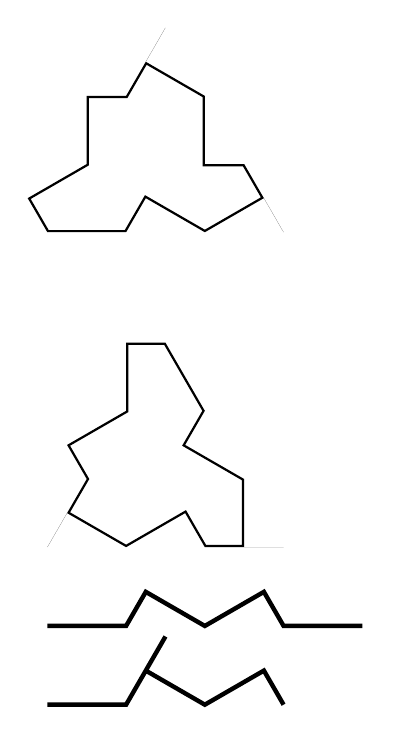
\begin{tikzpicture}
\pic[draw,subcluster H];
\pic[draw,subcluster T,at={(0,-4)}];
\pic[draw,subcluster P,at={(0,-5)}];
\pic[draw,subcluster F,at={(0,-6)}];
\end{tikzpicture}


\begin{tikzpicture}[
  every subcluster H/.style={draw, ultra thick},
  every subcluster T/.style={draw, ultra thick},
  every subcluster F/.style={draw=red}
]
\pic[subcluster H, name=A];
\pic[subcluster F, name=B, align with=A along b1];
\pic[subcluster F, name=C, align with=B along F];
\pic[subcluster F, name=D, align with=C along F];
\pic[subcluster H, name=E, align with=C along B using 1];
\pic[subcluster H, name=F, align with=D along B using 1];


\end{tikzpicture}



\end{document}
